% Métricas DORA em repositórios populares do GitHub
% Laboratório de Experimentação de Software — PUC Minas
%
% Compilação: requer o template oficial da SBC (sbc-template.sty, sbc-template.cls e
% as figuras do template) na mesma pasta. Veja artigo/README.md.
\documentclass[12pt]{article}

\usepackage{sbc-template}
\usepackage{graphicx,url}
\usepackage[brazil]{babel}
\usepackage[utf8]{inputenc}
\usepackage{booktabs}
\usepackage{multirow}

% As figuras são geradas por `python -m analise` e não são editadas à mão.
\graphicspath{{../resultados/figuras/}}

\sloppy

\title{Métricas DORA em repositórios populares do GitHub:\\
       o que muda quando muda a definição}

\author{João Gabriel S. A. Almeida\inst{1}, Lucas F. Ribeiro\inst{1}, Vitor V. Silva\inst{1}}

\address{Instituto de Ciências Exatas e Informática --- Pontifícia Universidade
  Católica de Minas Gerais (PUC Minas)\\
  Belo Horizonte --- MG --- Brasil
  \email{\{integrante1,integrante2,integrante3\}@sga.pucminas.br}
}

\begin{document}

\maketitle

\begin{abstract}
We measured the four DORA metrics in 300 popular GitHub repositories that use GitHub
Actions, over the 2025 calendar year, from 18{,}389 releases and 20{,}117 CI failure
episodes. Using medians and IQR, the sample shows a median of 0.46 releases per week,
a lead time of 324.9 hours, a CI change failure rate of 0.056 and a recovery time of
4.94 hours. The central result is not any single value but their fragility: swapping one
operational definition reclassifies up to 31.3\% of the repositories (weighted
$\kappa = 0.51$), and changing the \emph{metric variant} moves the classification far
more than changing the \emph{deploy unit}. We also found that 86.3\% of repositories
change their overall DORA category if a single metric moves one band, which means a
disagreement between two independent executions does not imply a calculation error.
\end{abstract}

\begin{resumo}
Medimos as quatro métricas DORA em 300 repositórios populares do GitHub que usam GitHub
Actions, na janela de 2025, a partir de 18.389 releases e 20.117 episódios de falha de
CI. Com mediana e IQR, a amostra apresenta 0,46 release por semana, lead time de 324,9
horas, change failure rate de CI de 0,056 e tempo de recuperação de 4,94 horas. O
resultado central não é nenhum desses valores, e sim a fragilidade deles: trocar uma
definição operacional reclassifica até 31,3\% dos repositórios ($\kappa$ ponderado de
0,51), e mudar a \emph{variante da métrica} desloca a classificação muito mais do que
mudar a \emph{unidade de deploy}. Encontramos ainda que 86,3\% dos repositórios mudam de
categoria geral se uma única métrica andar um degrau, o que significa que uma divergência
entre duas execuções independentes não implica erro de cálculo.
\end{resumo}

\section{Introdução}

As métricas DORA --- \emph{deployment frequency}, \emph{lead time for changes},
\emph{change failure rate} e \emph{time to restore service} --- tornaram-se a referência
para avaliar desempenho de entrega de software \cite{forsgren2018,dora2024}. Elas foram
formuladas a partir de questionários respondidos por equipes sobre os seus próprios
processos, com acesso a pipelines de produção, incidentes e implantações. Aplicá-las a
repositórios open-source exige traduzir cada conceito para artefatos que o GitHub
expõe publicamente, e é nessa tradução que mora o problema deste trabalho: ``deploy''
vira \emph{release}, ``falha em produção'' vira \emph{workflow run} vermelho, e
``restaurar o serviço'' vira o próximo run verde. Nenhuma dessas equivalências é exata.

Este artigo mede as quatro métricas em 300 repositórios populares do GitHub que usam
GitHub Actions e, principalmente, mede o quanto o resultado depende dessas escolhas de
tradução. Respondemos oito questões de pesquisa: as RQ 01 a 04 quantificam cada métrica;
a RQ 05 testa a correlação entre frequência de entrega e taxa de falha; a RQ 06 procura
fatores associados ao desempenho; a RQ 07 troca as definições operacionais e mede quanto
a classificação se move; e a RQ 08 explora uma métrica adicional de retrabalho.

Antes de olhar os dados, registramos quatro hipóteses informais, que a Seção
\ref{sec:discussao} confronta com os resultados:

\begin{description}
  \item[H1] Projetos populares entregam com frequência alta, concentrando-se nas faixas
    \emph{Elite} e \emph{High} de \emph{deployment frequency}.
  \item[H2] As duas variantes de lead time (por release e por commit) produzem valores
    próximos, já que medem o mesmo intervalo por caminhos diferentes.
  \item[H3] Velocidade e estabilidade não são um \emph{trade-off}: quem entrega mais
    vezes não falha mais, como sustenta o relatório DORA.
  \item[H4] As conclusões são robustas à definição operacional escolhida; trocar
    \emph{release} por \emph{tag}, ou uma variante de métrica por outra, muda pouco.
\end{description}

O código, os dados e todas as tabelas e figuras deste artigo são reexecutáveis por um
único comando e estão em
\url{https://github.com/Paulooassis/Laboratorio-03-medicao-de-software}.

\section{Metodologia}
\label{sec:metodologia}

\subsection{Seleção da amostra}

Buscamos repositórios públicos com pelo menos 1.001 estrelas e aplicamos, em ordem de
custo de API, os critérios de inclusão: usar GitHub Actions, ter no mínimo 5 releases e
50 \emph{workflow runs} válidos na janela de 1º de janeiro a 31 de dezembro de 2025. O
funil partiu de 1.025 candidatos e chegou a 300 repositórios; o descarte mais frequente
foi ``menos de 5 releases na janela'', com 511 repositórios (Tabela \ref{tab:funil}).

\begin{table}[ht]
\centering
\caption{Funil de seleção da amostra.}
\label{tab:funil}
\begin{tabular}{lr}
\toprule
\textbf{Etapa} & \textbf{Repositórios} \\
\midrule
Candidatos recebidos da busca & 1.025 \\
Repositórios únicos avaliados & 1.021 \\
Com GitHub Actions & 917 \\
Com 5 ou mais releases na janela & 406 \\
Com 50 ou mais workflow runs válidos & 300 \\
\midrule
\textbf{Incluídos na amostra} & \textbf{300} \\
\bottomrule
\end{tabular}
\end{table}

\subsection{Definições operacionais e as duas variantes obrigatórias}

A combinação de referência, que chamamos \textbf{C1}, usa: \emph{deploy} = release
publicada; \emph{lead time} pela variante (a), do commit mais antigo do intervalo entre
releases até a publicação; \emph{change failure rate} pela variante (a), falhas sobre
\emph{workflow runs} considerados; e tempo de recuperação da primeira falha até o
primeiro sucesso do mesmo workflow. As variantes alternativas são o lead time (b), por
commit, e o CFR (b), por entrega --- uma release é considerada falha quando é seguida,
em até sete dias, por uma release corretiva da mesma linha \emph{major.minor}.

A C1 usa estritamente a variante (a) do lead time. Um repositório sem lead time (a) fica
sem classificação nessa métrica, em vez de cair para a variante (b): como a RQ 07 compara
a C1 com a C4, que difere dela apenas pelas variantes das métricas, aceitar o
\emph{fallback} colocaria repositórios híbridos dentro da referência.

\subsection{Estatística}

Todas as métricas são resumidas por \textbf{mediana e IQR}, nunca por média e
desvio-padrão: as distribuições são assimétricas e de cauda longa, como mostra a Figura
\ref{fig:violino}. Correlações usam Spearman ($\rho$), por não exigir linearidade;
reportamos Pearson ($r$) apenas como contraste. Comparações entre grupos usam
Kruskal-Wallis com correção de Holm para múltiplas comparações, $\varepsilon^2$ como
tamanho de efeito e Cliff's $\delta$ nos pares, com a interpretação de
\citeonline{romano2006}. A concordância entre classificações usa kappa ponderado linear,
interpretado por \citeonline{landis1977}.

Nada é estimado para fechar conta. Release sem intervalo confiável de commits não entra
no lead time e é contada por motivo; release publicada nos últimos sete dias da janela
não tem sete dias observados e fica fora do denominador do CFR (b); episódio de falha sem
sucesso posterior é censurado e não entra na mediana de recuperação. Todos esses totais
são reportados junto dos resultados.

A análise inteira é reexecutável a partir dos CSVs publicados, sem refazer a coleta, com
\texttt{python -m analise}; cada número citado neste artigo vem de um arquivo em
\texttt{resultados/}.

\section{Resultados}
\label{sec:resultados}

Esta seção apresenta os números sem interpretá-los; a leitura vai para a Seção
\ref{sec:discussao}. Todos os valores vêm de \texttt{resultados/}, gerado por
\texttt{python -m analise} sobre 300 repositórios, 18.389 releases e 20.117 episódios de
falha.

\subsection{RQ 01 a 04: as quatro métricas}

A Tabela \ref{tab:sintese} reúne mediana, quartis e IQR de cada métrica e variante, e a
Figura \ref{fig:violino} mostra a forma das distribuições. As quatro são fortemente
assimétricas: o lead time (a) vai de 1,2 h a mais de 50.000 h, com IQR de 880 h.

\begin{table}[ht]
\centering
\caption{Síntese das RQ 01 a 04: mediana, quartis e IQR por métrica e variante.}
\label{tab:sintese}
\small
\begin{tabular}{llrrrrr}
\toprule
\textbf{Métrica} & \textbf{Variante} & \textbf{n} & \textbf{Mediana} & \textbf{Q1} &
\textbf{Q3} & \textbf{IQR} \\
\midrule
Deployment frequency (rel./sem.) & única & 300 & 0,46 & 0,23 & 1,00 & 0,77 \\
\midrule
\multirow{2}{*}{Lead time (horas)} & (a) release & 300 & 324,91 & 116,73 & 996,90 & 880,17 \\
 & (b) commit & 300 & 411,81 & 128,16 & 1.844,33 & 1.716,16 \\
\midrule
\multirow{2}{*}{Change failure rate} & (a) CI & 300 & 0,056 & 0,013 & 0,133 & 0,120 \\
 & (b) entrega & 300 & 0,269 & 0,105 & 0,500 & 0,395 \\
\midrule
\multirow{2}{*}{Recuperação (horas)} & recuperados & 264 & 4,94 & 1,75 & 18,75 & 17,00 \\
 & limite inferior & 268 & 5,22 & 1,82 & 22,22 & 20,40 \\
\bottomrule
\end{tabular}
\end{table}

\begin{figure}[ht]
\centering
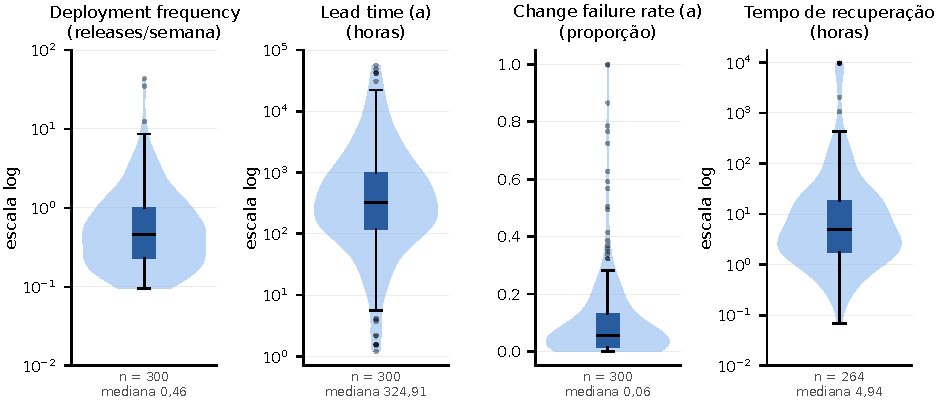
\includegraphics[width=\textwidth]{artigo_violino_metricas.pdf}
\caption{Distribuição das quatro métricas da C1. Violino para a forma, boxplot interno
para mediana e IQR. Unidades diferentes não dividem eixo: cada métrica tem seu painel, e
três delas estão em escala logarítmica.}
\label{fig:violino}
\end{figure}

\textbf{Censura e casos excluídos.} No lead time, 3.052 das 18.389 releases (16,6\%)
ficaram fora por motivo explícito: 3.026 por não trazerem commits novos em relação à
release anterior, 23 por não terem release anterior, 2 por \texttt{compare} com 404 e 1
por erro de \texttt{compare}. Nenhuma foi estimada ou tratada como intervalo zero. No
CFR (b), 246 releases publicadas nos últimos sete dias da janela ficaram fora do
denominador, em vez de contarem como sucesso, restando 18.143 avaliadas, das quais 10.974
falharam. No CFR (a) entraram 730.432 \emph{workflow runs} e ficaram de fora 60.959,
cancelados, em andamento ou com conclusão desconhecida. Na recuperação, dos 20.117
episódios de falha, 19.921 foram recuperados, 196 ficaram censurados e 124 com datas
contraditórias; 36 dos 300 repositórios não têm nenhum episódio recuperado e consistente,
e por isso ficam sem mediana. A proporção censurada por repositório tem mediana 0,00 e Q3
0,029. Tratando cada censurado como recuperado no fim da observação --- um limite
inferior do viés --- a mediana sobe de 4,94 h para 5,22 h, uma diferença de 0,28 h.

\subsection{Classificação DORA de referência (C1)}

A Tabela \ref{tab:c1} traz a distribuição das categorias. O CFR (a) concentra 234 dos 300
repositórios em \emph{Elite}; a classificação geral concentra-se em \emph{Medium} (154) e
\emph{High} (110), com apenas 9 \emph{Elite} e 27 \emph{Low}.

\begin{table}[ht]
\centering
\caption{Distribuição das categorias DORA na combinação C1 (300 repositórios).}
\label{tab:c1}
\small
\begin{tabular}{lrrrrr}
\toprule
\textbf{Métrica} & \textbf{Elite} & \textbf{High} & \textbf{Medium} & \textbf{Low} &
\textbf{Sem class.} \\
\midrule
Deployment frequency & 6 & 69 & 152 & 73 & 0 \\
Lead time (a) & 25 & 81 & 93 & 101 & 0 \\
Change failure rate (a) & 234 & 47 & 8 & 11 & 0 \\
Tempo de recuperação & 33 & 181 & 33 & 21 & 32 \\
\midrule
\textbf{Classificação geral} & \textbf{9} & \textbf{110} & \textbf{154} & \textbf{27} & \textbf{0} \\
\bottomrule
\end{tabular}
\end{table}

\subsection{RQ 05: frequência de entrega e taxa de falha}

Com o CFR (a), a correlação é desprezível e não significativa ($\rho = 0{,}071$,
$p = 0{,}222$, $n = 300$). Com o CFR (b), é moderada e fortemente significativa
($\rho = 0{,}615$, $p = 1{,}2 \times 10^{-32}$). A Figura \ref{fig:dispersao} mostra as
duas dispersões lado a lado.

\begin{figure}[ht]
\centering
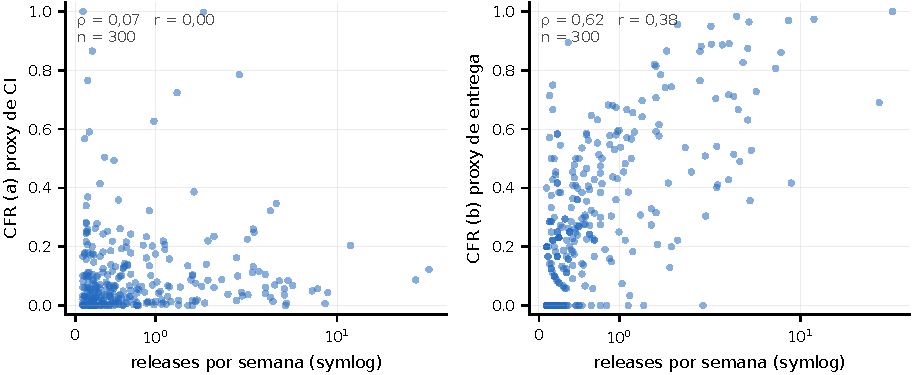
\includegraphics[width=\textwidth]{artigo_dispersao_df_cfr.pdf}
\caption{Frequência de entrega contra as duas variantes do CFR. À esquerda, o proxy de CI
não mostra relação; à direita, o proxy de entrega mostra associação positiva forte. Em
ambos os painéis, $\rho$ de Spearman e $r$ de Pearson.}
\label{fig:dispersao}
\end{figure}

O diagnóstico da janela de sete dias explica o segundo coeficiente: entre os
repositórios do quartil inferior de frequência, o intervalo mediano entre releases é de
27,9 dias e apenas 25,0\% dos intervalos cabem em sete dias; no quartil superior, o
intervalo mediano é de 1,39 dia e 87,7\% cabem na janela.

A Figura \ref{fig:correlacao} generaliza a análise para todos os pares de métricas, com
Spearman e Pearson lado a lado.

\begin{figure}[ht]
\centering
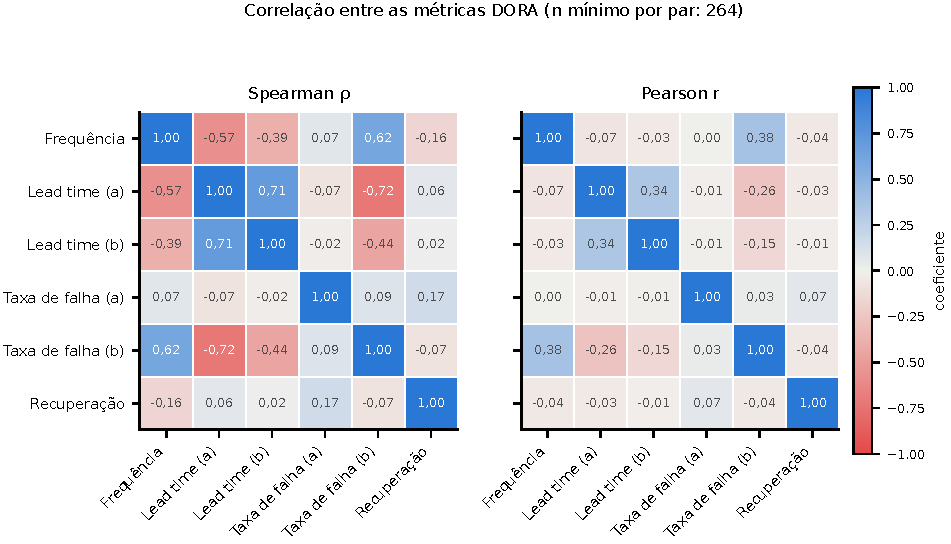
\includegraphics[width=\textwidth]{artigo_correlacao.pdf}
\caption{Correlação entre as métricas. O painel de Pearson é visivelmente mais pálido: em
DF $\times$ LT (a), $\rho = -0{,}57$ contra $r = -0{,}07$. As associações são monótonas,
não lineares.}
\label{fig:correlacao}
\end{figure}

\subsection{RQ 06: fatores associados ao desempenho}

Após a correção de Holm, quatro testes rejeitam a hipótese nula: linguagem contra
frequência de entrega ($\varepsilon^2 = 0{,}113$, efeito médio) e contra lead time (a)
($\varepsilon^2 = 0{,}164$, médio); número de contribuidores contra frequência
($\varepsilon^2 = 0{,}046$, pequeno) e contra lead time (a)
($\varepsilon^2 = 0{,}100$, médio). Estrelas não se associam a nenhuma das quatro
métricas após a correção. O fator idade não pôde ser testado: a estratificação não
produziu dois grupos válidos.

\subsection{RQ 07: sensibilidade às definições operacionais}

A Tabela \ref{tab:rq07} mostra o percentual de repositórios que mudam de categoria entre
cada par de combinações e o kappa ponderado correspondente.

\begin{table}[ht]
\centering
\caption{RQ 07: mudança de categoria geral entre combinações ($n = 300$).}
\label{tab:rq07}
\small
\begin{tabular}{llrrl}
\toprule
\textbf{Par} & \textbf{O que muda} & \textbf{Mudaram} & \textbf{\%} &
\textbf{$\kappa$ ponderado} \\
\midrule
C1 $\times$ C2 & unidade e variantes & 94 & 31,3 & 0,506 (moderada) \\
C1 $\times$ C3 & unidade (tag) & 73 & 24,3 & 0,651 (substancial) \\
C1 $\times$ C4 & só as variantes & 85 & 28,3 & 0,546 (moderada) \\
C2 $\times$ C4 & só a unidade & 22 & 7,3 & 0,878 (quase perfeita) \\
\bottomrule
\end{tabular}
\end{table}

Por métrica, o Change Failure Rate é o que mais se move: entre C1 e C2 muda em 72,3\% dos
repositórios, com $\kappa = -0{,}015$ --- concordância nula. A mediana do CFR passa de
0,056 na C1 para 0,274 na C2, um aumento de 3,88 vezes.

\subsection{RQ 08: taxa de retrabalho}

A taxa de retrabalho tem mediana 0,70 (IQR 0,41, $n = 300$): 12.020 das 18.366 releases
avaliadas foram classificadas como corretivas pela heurística v1. Sua correlação com o
CFR (b) é fraca ($\rho = 0{,}359$, $p = 1{,}5 \times 10^{-10}$). Avaliada contra a
amostra-ouro, a heurística v1 tem precisão 0,696, \emph{recall} 0,824 e F1 0,754.

\subsection{Fragilidade da classificação}

Em 259 dos 300 repositórios (86,3\%), mover uma única métrica um degrau muda a
classificação geral; em 53 a métrica mais próxima está a 5\% ou menos de um limite de
faixa, e em 31 as duas condições valem ao mesmo tempo. O caso mais extremo é
\texttt{ultralytics/ultralytics}, a 0,06\% do limite de 24 h do lead time.

\section{Discussão}
\label{sec:discussao}

\subsection{As hipóteses da Introdução contra os resultados}

\begin{table}[ht]
\centering
\caption{As oito hipóteses informais registradas antes da análise, uma por RQ.}
\label{tab:hipoteses}
\small
\begin{tabular}{p{0.7cm}p{4.4cm}p{5.4cm}l}
\toprule
 & \textbf{Hipótese} & \textbf{Resultado} & \textbf{Veredito} \\
\midrule
H1 & Frequência alta, em \emph{Elite}/\emph{High} &
     Mediana de 0,46 release/semana (\emph{Medium}); 6 \emph{Elite} e 69
     \emph{High} contra 152 \emph{Medium} e 73 \emph{Low} & Refutada \\
H2 & As variantes de lead time são próximas &
     Medianas de 324,9 h e 411,8 h; $\rho = 0{,}71$, mas IQR de 880 h contra 1.716 h &
     Parcial \\
H3 & CFR baixo e variantes concordantes &
     CFR (a) mediana 0,056 (\emph{Elite}), mas as variantes discordam em 72,3\% dos
     repositórios, com $\kappa = -0{,}015$ & Parcial \\
H4 & Recuperação abaixo de um dia &
     Mediana de 4,94 h; 181 dos 300 em \emph{High} e 33 em \emph{Elite} &
     Confirmada \\
H5 & Sem \emph{trade-off} velocidade × estabilidade &
     Confirma-se com o CFR (a) ($\rho = 0{,}07$); com o CFR (b), $\rho = 0{,}62$ por
     artefato de construção & Parcial \\
H6 & Estrelas associadas a melhor desempenho &
     Nenhuma das quatro métricas se associa a estrelas após Holm; linguagem e
     contribuidores, sim & Refutada \\
H7 & Conclusões robustas à definição &
     Até 31,3\% mudam de categoria; trocar a variante pesa quase 4× mais que trocar a
     unidade & Refutada \\
H8 & Retrabalho baixo e próximo do CFR (b) &
     Mediana de 0,70 (alta) e correlação apenas fraca com o CFR (b)
     ($\rho = 0{,}36$) & Refutada \\
\bottomrule
\end{tabular}
\end{table}

\subsection{Velocidade e Lead Time (H1 e H2)}

A H1 foi \textbf{refutada}. A mediana de 0,46 release por semana equivale a uma entrega a
cada 15 dias e enquadra a amostra em \emph{Medium}, não em \emph{Elite} ou \emph{High}:
apenas 6 dos 300 repositórios publicam diariamente ou mais. Projetos open-source populares
operam em regime \emph{descontínuo} de releases, agrupando mudanças em lotes, mesmo quando
dispõem de automação madura de CI.

A H2 foi \textbf{parcialmente confirmada}, e o modo como ela falha é informativo. As duas
variantes correlacionam-se fortemente ($\rho = 0{,}71$), o que sustenta a expectativa de que
medem o mesmo fenômeno; mas divergem em escala e, sobretudo, em dispersão: a variante (b)
tem IQR de 1.716 h contra 880 h da (a). A razão é estrutural. A variante (a) é definida pelo
commit \emph{mais antigo} de cada release, enquanto a (b) é a mediana de \emph{todos} os
commits. Basta um commit antigo esquecido no intervalo --- um \emph{branch} retomado, um
\emph{cherry-pick}, um \emph{pull request} parado --- para a (a) subir sem que o ritmo de
trabalho tenha mudado. As duas respondem a perguntas distintas: a (a), "quanto tempo cabe
dentro de uma entrega"; a (b), "quanto tempo um commit típico espera para ser entregue".

\subsection{A Ilusão de Estabilidade do \emph{Proxy} de CI (H3)}

A H3 foi \textbf{parcialmente confirmada}: a taxa é de fato baixa pelo \emph{proxy} de CI
(mediana de 5,63\%, faixa \emph{Elite}, com 234 dos 300 repositórios nessa faixa), mas a
previsão de que as duas variantes concordariam está errada por larga margem --- elas
discordam de faixa em 72,3\% dos repositórios, com $\kappa = -0{,}015$.

A diferença não é de calibração, é de objeto. Uma execução de CI vermelha é, na maior parte
das vezes, um teste quebrado em um \emph{pull request}: barata, detectada antes da entrega e
frequentemente a prova de que o CI está fazendo o seu trabalho. Uma release seguida de uma
corretiva em até sete dias é um defeito que atravessou o pipeline e chegou ao usuário. O
\emph{proxy} de CI mede a \emph{barreira}; o de entrega mede o que \emph{passou} por ela.
Comparar qualquer um dos dois diretamente com as faixas do relatório DORA, que falam de
produção, induz a erro --- e o CFR (a), com 78\% da amostra em \emph{Elite}, sugere uma
estabilidade que não mediu.

\subsection{O Artefato de Construção do CFR de Entrega (H4 e H5)}

A H4 foi \textbf{confirmada}: a recuperação mediana de 4,94 h fica bem abaixo das 24 h
previstas, com 181 dos 300 repositórios em \emph{High} e 33 em \emph{Elite}. Uma \emph{build}
quebrada no \emph{default branch} é, de fato, tratada com prioridade.

A H5 é o ponto mais delicado do estudo. Com o \emph{proxy} de CI, a ausência de
\emph{trade-off} se confirma ($\rho = 0{,}07$, não significativo). Com o \emph{proxy} de
entrega, a correlação é positiva e moderada ($\rho = 0{,}62$), o que, lido ingenuamente,
contradiria o DORA e sugeriria que entregar mais causa mais falhas. O diagnóstico da janela
de sete dias mostra que a leitura é um \textbf{artefato de construção da própria métrica}:
no quartil superior de frequência, 87,7\% dos intervalos entre releases cabem em sete dias,
contra 25,0\% no quartil inferior. Quem publica a cada 1,4 dia quase sempre tem uma release
seguinte dentro da janela de observação da heurística e, portanto, muito mais chance de ser
marcado como falha; quem publica a cada 28 dias quase nunca tem. O numerador e o denominador
compartilham a mesma causa --- a cadência --- e o coeficiente mede cadência disfarçada de
estabilidade. Correlação não implica causalidade; aqui, sequer há correlação legítima a
interpretar.

\subsection{Fatores Estruturais e o Peso da Definição (H6, H7 e H8)}

A H6 foi \textbf{refutada} no ponto que previa: estrelas não se associam a nenhuma das
quatro métricas após a correção de Holm. A popularidade parece operar como indicador de
reputação, desacoplado do fluxo interno de engenharia. O que sobrevive são linguagem
($\varepsilon^2 = 0{,}164$ no lead time) e número de contribuidores
($\varepsilon^2 = 0{,}100$), ambos com efeito médio. Vale separar significância de
relevância: com $n = 300$, efeitos pequenos alcançam significância sem significar muito.

A H7 foi \textbf{refutada}, e o desenho das combinações permite dizer \emph{como}. Entre C2
e C4, que diferem apenas na unidade de deploy, somente 7,3\% dos repositórios mudam de
categoria ($\kappa = 0{,}878$). Entre C1 e C4, que diferem apenas nas variantes das métricas,
28,3\% mudam ($\kappa = 0{,}546$). Ou seja: \textbf{trocar a variante da métrica desloca a
classificação quase quatro vezes mais do que trocar a unidade de deploy}. A discussão sobre
se \emph{tag} ou release conta como deploy, que ocupa boa parte da literatura de mineração,
importa menos do que a escolha entre CFR de CI e CFR de entrega.

A H8 foi \textbf{refutada} nas duas partes: a taxa de retrabalho não é baixa (mediana de
70,0\%) e sua correlação com o CFR de entrega é apenas fraca ($\rho = 0{,}36$), embora ambas
derivem da mesma heurística. A explicação está na janela: o retrabalho conta toda release
corretiva do período, enquanto o CFR (b) só conta aquelas que \emph{seguem} outra release em
até sete dias. Repositórios que corrigem com calma produzem retrabalho alto e CFR (b) baixo.

\subsection{A Fragilidade das Fronteiras}

Soma-se a tudo isso um achado que não estava previsto em nenhuma hipótese: 86,3\% dos
repositórios mudam de categoria geral se uma única métrica avançar um degrau. A
classificação em faixas é uma discretização de medidas contínuas, e nada no método sinaliza
quem está na fronteira. Esse resultado nasceu de uma divergência relatada na replicação
cruzada (Seção \ref{sec:replicacao}) e reposiciona a interpretação de qualquer comparação de
categorias entre estudos.

\section{Ameaças à Validade}
\label{sec:ameacas}

A estrutura desta seção segue a taxonomia usual de ameaças em engenharia de software
experimental \cite{wohlin2012}. Cada ameaça é apoiada em uma evidência do próprio estudo e
acompanhada da mitigação adotada, ou da razão de não ter sido possível mitigá-la.

\textbf{Validade de Construto.} A equivalência entre release e deploy, e entre
\emph{workflow run} vermelho e falha de entrega, é uma aproximação inerente ao uso de
\emph{proxies}. A amostra-ouro mitiga parcialmente a primeira: 295 das 300 releases
rotuladas representam entregas reais ao usuário, 5 ficaram incertas e nenhuma foi rotulada
como "não" --- a suposição se sustenta nesta amostra. Ela permanece, porém, para as 95
releases de bibliotecas e \emph{frameworks}, em que publicar no registro não implica que
alguém atualizou a dependência. A segunda equivalência é o objeto da Seção
\ref{sec:discussao} e não foi mitigada, e sim \emph{medida}: as duas variantes do CFR
discordam em 72,3\% dos repositórios. A heurística corretiva que sustenta o CFR (b) tem
F1 de 0,754, com 55 falsos positivos e 27 falsos negativos, e superdetecta corretivas ---
marca 65,4\% das releases contra 51\% na rotulagem manual. Além disso,
\texttt{commit.author.date} é vulnerável a \emph{rebase} e \emph{squash merge}, que reescrevem
a data e distorcem o lead time sem relação com o esforço real; mitigamos apenas
contabilizando datas ausentes em vez de estimá-las, e mantendo valores negativos visíveis em
vez de descartá-los. Por fim, há uma ameaça ao próprio instrumento de validação: o consenso
da amostra-ouro foi consolidado em um arquivo único do grupo, e as planilhas individuais dos
três avaliadores não estão versionadas, o que impede recalcular o $\kappa$ de Fleiss e,
portanto, aferir a confiabilidade da rotulagem que sustenta o F1 relatado.

\textbf{Validade Interna.} O principal confundidor identificado é a própria cadência: um
repositório que publica com frequência tem mais oportunidades de ter uma release corretiva
dentro de sete dias, o que infla o CFR (b) independentemente da qualidade. Esse mecanismo
foi quantificado (87,7\% contra 25,0\% dos intervalos dentro da janela) e é reportado junto
do coeficiente, não omitido. Releases publicadas por robôs de automação ---
\emph{release-please}, \emph{semantic-release}, Dependabot --- entram como qualquer outra e
inflam a frequência de projetos que automatizaram a publicação; essa ameaça não foi mitigada,
pois não distinguimos autor humano de robô. Execuções agendadas são excluídas pelo filtro de
evento \texttt{push}, mas execuções com matriz de combinações contam como um único
\emph{run}. O truncamento no fim da janela foi tratado por censura explícita, e não por
descarte, em ambos os pontos em que ocorre: 196 episódios de recuperação (0,97\%) e 246
releases do CFR (b) (1,3\%).

\textbf{Validade Externa.} A amostra é deliberadamente estreita: repositórios públicos com
pelo menos 1.001 estrelas, que usam GitHub Actions, observados em uma única janela anual. O
funil dimensiona o recorte: 511 dos 1.021 candidatos avaliados caíram por publicar menos de
cinco releases em doze meses, e outros 103 por não usarem Actions. Os achados descrevem,
portanto, projetos populares, ativos e automatizados --- não o GitHub como um todo, e muito
menos desenvolvimento corporativo, onde o DORA foi formulado e onde "deploy" tem acesso a
dados de produção que aqui não existem. Pipelines em GitLab CI ou Jenkins estão fora do
alcance do instrumento. A janela única impede ainda qualquer afirmação de tendência: 2025 é
um retrato, não uma série temporal.

\textbf{Validade de Conclusão.} A família principal da RQ 06 executa 16 testes, e a correção
de Holm foi aplicada sobre ela; o efeito é observável --- estrelas contra frequência tem
$p = 0{,}0070$ bruto e $p = 0{,}0556$ corrigido, deixando de ser significativo. Todos os
testes são não paramétricos, o que protege as deduções contra a assimetria documentada na
Figura \ref{fig:violino}, e todos os tamanhos de efeito são reportados junto dos $p$-valores.
A análise exploratória por tipo de projeto apoia-se em 60 repositórios distribuídos em três
tipos, e está declarada como exploratória por isso. A mediana de recuperação usa apenas
episódios recuperados e, por construção, subestima o tempo real, já que os episódios mais
longos são justamente os que não terminam na janela; publicamos o limite inferior que trata
cada censurado como recuperado no fim da observação (5,22 h contra 4,94 h) para dimensionar
esse viés. O $n$ difere entre métricas (264 na recuperação contra 300 nas demais), o que
impede comparações diretas de dispersão entre elas. Por fim, as faixas DORA produzem muitos
empates de fronteira: 86,3\% dos repositórios estão a um degrau de outra categoria, de modo
que comparações de categoria entre estudos precisam reportar essa proximidade, sob pena de
atribuir a erro de cálculo o que é efeito da discretização.

\section{Replicação Cruzada}
\label{sec:replicacao}

Em conformidade com as diretrizes do estudo, a replicação ocorreu nas duas direções sobre
uma subamostra determinística de 30 repositórios sorteada com semente fixa e documentada,
seguindo apenas o \texttt{README} publicado de cada lado.

\subsection{Como Replicadores}

Executamos o \emph{pipeline} do grupo sorteado no commit \texttt{73b739f}, em macOS 27.0.1
(arm64) com Python 3.14.0, em ambiente virtual novo e sem nenhum cache prévio. A subamostra
foi sorteada sobre o conjunto ordenado e deduplicado dos 300 repositórios do dataset
original deles, com o \emph{hash} SHA-256 do CSV de origem registrado junto da lista, de
modo que o sorteio seja refazível por qualquer pessoa --- inclusive pelo grupo autor ao
responder as Issues.

\textbf{O estudo foi executável}, com uma ressalva de escopo. Clone, instalação das nove
dependências e o modo de estimativa de consumo de API funcionaram sem atrito, somando menos
de dois minutos. A execução completa levou \textbf{42 min 20 s}, dos quais 38 min 38 s
(91\%) foram espera da API, consumindo cerca de 1.676 requisições para 30 repositórios ---
aproximadamente 2,5 vezes a projeção linear da própria estimativa do \emph{pipeline}. Todos
os artefatos prometidos foram produzidos e a suíte de testes do grupo passou integralmente
(159 testes, 77\% de cobertura).

A ressalva é relevante para a própria viabilidade da replicação: \textbf{não existe forma,
documentada ou não, de executar aquele \emph{pipeline} sobre um conjunto dado de
repositórios}. A etapa de seleção sempre refaz a busca por faixas de estrelas, que depende
da contagem de estrelas no instante da execução e, portanto, não é estável entre execuções.
Para rodar sobre a subamostra foi necessário ler o código-fonte, descobrir que as etapas
seguintes consomem um CSV intermediário e escrevê-lo manualmente --- isto é, sair do
\texttt{README}. Seguindo estritamente a documentação, a replicação cruzada como o estudo a
define não é executável naquele \emph{pipeline}.

Quanto aos valores, a reprodução foi praticamente exata: a diferença relativa mediana foi de
\textbf{0,0\% nas sete métricas} comparadas, com concordância de categoria de 100\% em
frequência, lead time e CFR, e de 91,3\% na recuperação ($\kappa$ ponderado de 0,907). As
divergências concentram-se em repositórios com poucos episódios de falha, em que um único
episódio a mais ou a menos desloca a mediana; o maior desvio relativo observado na
recuperação chega a 945\%, em um repositório com baixa contagem de episódios. Abrimos quatro
Issues no repositório do grupo autor: uma de execução e documentação, referente à ausência de
parâmetro para a subamostra, e três de documentação --- links apontando para o disco local de
um dos autores, instalação sem ambiente virtual e contagem de colunas desatualizada.

\subsection{Como Autores}

Recebemos três Issues do grupo replicador, todas procedentes e todas corrigidas antes do
prazo, e todas registradas no GitHub Projects do grupo.

A primeira relatava que o comando de análise falhava em um clone limpo, porque os CSVs do
estudo não estavam versionados na \emph{branch} principal --- existiam apenas em uma
\emph{branch} seis commits à frente, nunca integrada. Corrigimos publicando os três CSVs, de
modo que a análise passou a ser reexecutável a partir de um clone limpo, sem token e sem
refazer a coleta.

A segunda apontava a ausência de um parâmetro para executar sobre a subamostra --- exatamente
a mesma lacuna que havíamos encontrado no \emph{pipeline} deles. Acrescentamos uma opção que
recebe a lista de repositórios e substitui a busca por estrelas, preservando os critérios de
inclusão: um repositório da lista que não os atenda continua aparecendo no funil como
excluído, com o motivo registrado.

A terceira relatava que um repositório mudara de categoria geral entre o dataset publicado e
a reexecução. A investigação mostrou que \textbf{não havia erro de cálculo em nenhum dos dois
lados}: o repositório está 1,87 h acima do limite de 168 h entre \emph{Medium} e \emph{Low} no
tempo de recuperação --- 1,10\% do valor --- e, como a categoria geral é a mediana das quatro
notas arredondada para baixo, mover uma única métrica um degrau basta para alterá-la. Essa
Issue motivou a análise de fragilidade de fronteira relatada na Seção \ref{sec:resultados} e
a ameaça à validade de conclusão correspondente.

\subsection{O que a Replicação Mudou no Estudo}

Além das três correções, a tentativa de reproduzir a comparação revelou um defeito que
\emph{nenhuma} das Issues havia apontado: o módulo de análise esperava nomes de coluna que o
\emph{pipeline} de coleta não escreve. Como coluna ausente é tratada como valor ausente por
contrato, a análise lia o CSV real \textbf{sem erro algum e devolvia estatísticas vazias}. A
falha ruidosa relatada pelo grupo replicador encobria uma falha silenciosa; corrigida a
primeira, a segunda tornou-se visível. É o argumento mais concreto que este trabalho produziu
em favor da replicação cruzada como prática.

\section{Conclusão}
\label{sec:conclusao}

Mineramos as quatro métricas DORA em 300 repositórios open-source populares que usam GitHub
Actions, ao longo da janela anual de 2025. A amostra revelou desenvolvimento organizado em
ciclos discretos --- mediana de 0,46 release por semana e lead time por release de 324,9 h
(13,5 dias) --- desafiando a premissa de entrega contínua diária herdada do contexto
corporativo; a maior parte concentra-se em \emph{Medium} (154) e \emph{High} (110), com apenas
9 em \emph{Elite}. A estabilidade percebida varia drasticamente conforme a lente: o
\emph{proxy} de CI sugere maturidade \emph{Elite} (5,63\%), o de entrega indica correção
frequente (26,92\%), e os dois discordam de faixa em 72,3\% dos repositórios.

O achado central não é nenhum desses valores, e sim a sua dependência de escolhas que o
método não torna visíveis. Até 31,3\% dos repositórios migram de categoria entre combinações
e --- graças ao desenho que separa os dois efeitos --- trocar a \textbf{variante da métrica}
desloca a classificação quase quatro vezes mais do que trocar a \textbf{unidade de deploy}
(28,3\% contra 7,3\%). Somado a isso, 86,3\% mudam de categoria se uma única métrica avançar um
degrau, porque as faixas discretizam medidas contínuas sem sinalizar quem está na fronteira.

Decorrem daí três consequências práticas: relatar uma classificação DORA sem explicitar as
definições adotadas não é informativo; o CFR calculado sobre falhas de CI não é comparável às
faixas do relatório DORA, que tratam de produção; e comparações de categoria entre estudos ou
execuções precisam reportar quantos repositórios estavam próximos de um limite, sob pena de
atribuir a erro de cálculo o que é efeito da discretização --- lição que a replicação cruzada
nos impôs na prática.

Como trabalhos futuros, propõem-se validar a heurística corretiva em uma segunda amostra
rotulada, independente daquela em que foi calibrada; estender a observação para além de uma
janela anual, permitindo falar de tendência; e substituir as faixas discretas por uma medida
contínua de desempenho, que não reproduza a fragilidade de fronteira documentada aqui.

\vspace{0.2cm}
\noindent\textbf{Disponibilidade.} Código, dados, dicionário de dados e todas as tabelas e
figuras deste artigo estão em
\url{https://github.com/Paulooassis/Laboratorio-03-medicao-de-software}, reexecutáveis com
\texttt{python -m analise}. O acompanhamento de Issues e sprints está em
\url{https://github.com/Paulooassis/Laboratorio-03-medicao-de-software/projects}.


\bibliographystyle{sbc}
\bibliography{referencias}

\end{document}
